% !TEX root =  ../Dissertation.tex
\chapter{Implementation}
\begin{figure}[h] % 'h' means 'here' - places the figure where it's defined
    \centering
    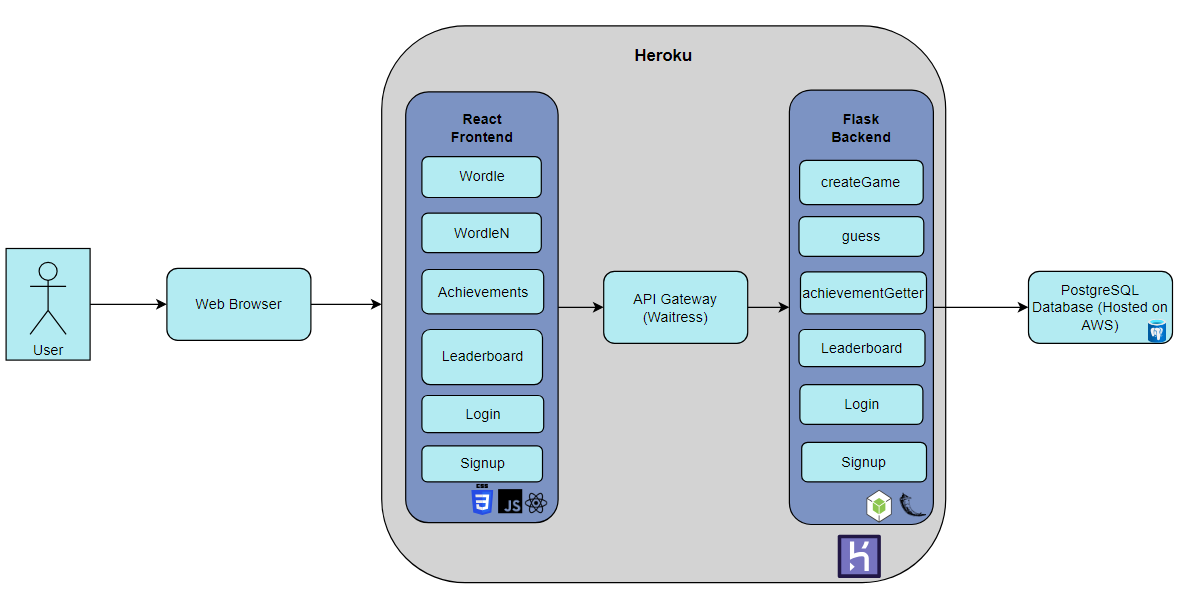
\includegraphics[width=\textwidth]{Architecture_Diagram_New_New.png
    } % Replace with your image file
    \caption{Architecture Diagram}
    \label{fig:example}
\end{figure}

The web application's front end uses React.js. After researching various front-end frameworks, the component-based architecture of React emerged as a natural choice, particularly for implementing keyboard functionality. This approach seemed well-suited for the different use cases anticipated for the keyboard, mainly because potential users had discussed the idea of an extended Wordle version.
Another significant consideration was React's status as one of the most widely used front-end frameworks in modern web development. The popularity of React presented an opportunity to enhance skills in web development beyond the scope of what was covered in the course. Additionally, React was chosen to facilitate learning and development in CSS, offering a chance to improve front-end development capabilities beyond creating websites with a Flask backend, using HTML and CSS with Bootstrap. Although these tools might have achieved a similar aesthetic outcome, the goal was also to expand expertise in front-end technologies.
A different framework was considered for the application's backend. However, after conducting research, it was determined that switching to Django would not offer enough challenges to significantly contribute to personal growth and development. Conversely, transitioning to an entirely different programming language was deemed too daunting, especially when concurrently learning JavaScript, React, and CSS.
The website's planned design also required many database calls. The database would store guesses, answers, and user data, just to name a few. For this approach to web development, SQLAlchemy seemed appropriate. Using the ORM style of SQL calls gave the ability to interact with the database in a Pythonic manner and let the calls and insertion of data be weaved into the code, as almost every call to the backend required some call to the database.

\section{Database}
\begin{figure}[h] % 'h' means 'here' - places the figure where it's defined
    \centering
    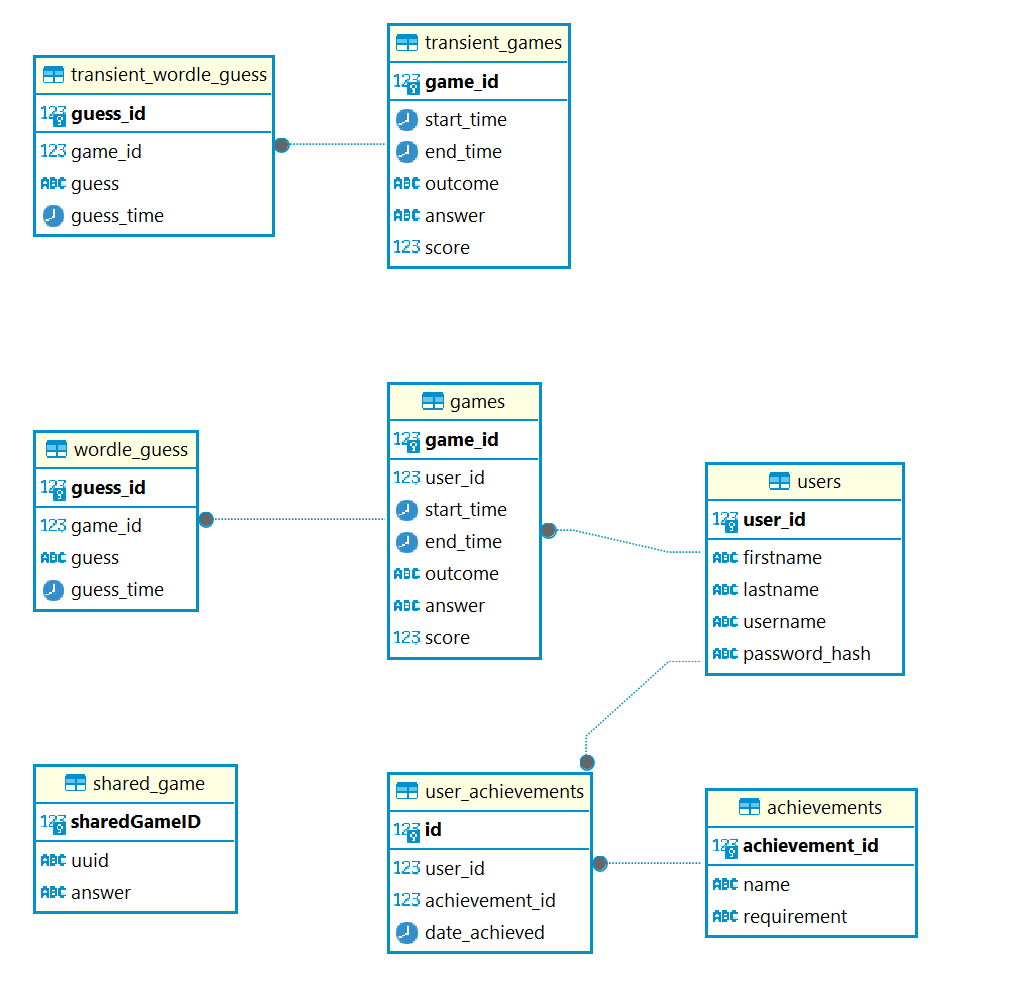
\includegraphics[width=\textwidth]{Database_Schema_Diagram.png} % Replace with your image file
    \caption{Database Schema Diagram}
    \label{fig:example}
\end{figure}
The database schema illustrates the system designed to handle both Wordle with no login and The Gauntlet
\subsection{Transient Mode (Wordle with no login)}
Two main tables are used in the transient mode: transientGames and transientWordleGuess.
\begin{itemize}
    \item transientGames
        \begin{itemize}
        \item gameId: A unique identifier for each game played.
        \item startTime and endTime: Timestamp fields that record when the game started and ended.
        \item Outcome: Stores the outcome of the game played.
        \item Answer: Stores the correct answer of the game.
        \item Score: Stores how well the user did in the game.
        \end{itemize}
    \item transientWordleGuess
        \begin{itemize}
        \item guessId: A unique id for each guess.
        \item gameId: A foreign key that links each guess to the corresponding game in the transientGames table.
        \item Guess: Stores the players guess.
        \item guessTime: Stores the time when the player guesses
        \end{itemize}
    \end{itemize}
    
\subsection{The Gauntlet}
\begin{itemize}
\item users
    \begin{itemize}
    \item userId: Primary key that identifies each user.
    \item firstName, lastName, username, passwordHash: All fields that store personal information of each user.
    \end{itemize}
\item games
    \begin{itemize}
    \item gameId: Primary key that identifies each user.
    \item userId: A foreign key which links the game to a specific user.
    \item startTime and endTime: Timestamps that indicate the time of the first guess and the time of the final guess.
    \item outcome: Stores the result of the game.
    \item answer: Stores the correct answer for the game.
    \item Score: stores the score achieved by the user.
    \end{itemize}
\item wordleGuess
    \begin{itemize}
    \item guessId: Primary key that identifies the guess.
    \item gameId: A foreign key that links the guess to the corresponding game in the games table.
    \item guess: stores the guess made by a user.
    \item guessTime: Timestamps when the guess was made.
    \end{itemize}
\item sharedGame
    \begin{itemize}
    \item sharedGameId: The primary key for instances of a shared game.
    \item uuid: Stores the unique identifier of each shared game.
    \item answer: The correct answer for the shared game.
    \end{itemize}
\item userAchievements
    \begin{itemize}
    \item id: The primary key for the user achievements table.
    \item userId: The foreign key that links achievements to a specific user.
    \item achievementId: A foreign key that links to a specific achievement on the achievement table.
    \item dateAchieved: The date when the achievement was earned by the user.
    \end{itemize}
\item achievements
    \begin{itemize}
    \item achievementId: The primary key for the achievements table.
    \item name: The name of the achievement
    \item requirement: The criteria that needs to be met to earn the achievement.
    \end{itemize}
\end{itemize}

\section{Unit Testing}
In this project, unit tests were implemented for key components across both the front end and back end. The backend unit tests were written using the unittest framework in Python, focusing on the application's core logic and APIs, such as the Wordle game logic and user authentication mechanisms. For example, the TestParseResult class in testServer.py contains several test cases that verify the correctness of the parseResult function, ensuring that it accurately evaluates the user's guesses against the correct Wordle answer.

\begin{lstlisting}[style=python, caption={The parseResult functions unit tests}]
class TestParseResult(unittest.TestCase):
    def test_all_correct(self):
        guess = "apple"
        answer = "apple"
        expected_result = ['correct', 'correct', 'correct', 'correct', 'correct']
        self.assertEqual(parseResult(guess, answer), expected_result)

    def test_some_present(self):
        guess = "apple"
        answer = "apply"
        expected_result = ['correct', 'correct', 'correct', 'correct', 'absent']
        self.assertEqual(parseResult(guess, answer), expected_result)

    def test_some_absent(self):
        guess = "apple"
        answer = "quick"
        expected_result = ['absent', 'absent', 'absent', 'absent', 'absent']
        self.assertEqual(parseResult(guess, answer), expected_result)

    def test_mixed(self):
        guess = "apple"
        answer = "plead"
        expected_result = ['present', 'present', 'absent', 'present', 'present']
        self.assertEqual(parseResult(guess, answer), expected_result)
\end{lstlisting}

Similarly, the front end unit tests were implemented using the @testing-library/react and jest frameworks, ensuring that the React components behave as expected under various conditions. Components such as Leaderboard, Achievements, and Wordle were tested. For instance, the Achievements.test.js file includes tests that simulate user interactions and validate that achievements are correctly fetched and displayed based on the user's progress. These tests help ensure that the front end functions correctly in isolation and integrates smoothly with the backend services.

\begin{lstlisting}[style=python, caption={Achievement frontend unit testing}]
describe('Achievements Component', () => {
    const mockUser = { token: 'mock-token' };
    beforeEach(() => {
        global.fetch = jest.fn();
    });
    afterEach(() => {
        jest.resetAllMocks();
    });
    it('fetches and displays achievements', async () => {
        const mockUserAchievements = ['Achievement 1'];
        const mockAllAchievements = ['Achievement 1', 'Achievement 2'];
        fetch.mockImplementationOnce(() =>
            Promise.resolve({
                ok: true,
                json: () => Promise.resolve(mockUserAchievements),
            })
        );
        fetch.mockImplementationOnce(() =>
            Promise.resolve({
                ok: true,
                json: () => Promise.resolve(mockAllAchievements),
            })
        );
        await act(async () => {
            render(<Achievement user={mockUser} />);
        });
        await waitFor(() => {
            expect(screen.getByText('Achievement 1')).toBeInTheDocument();
            expect(screen.getByText('Achievement 2')).toHaveClass('not-achieved');
        });
    });
    it('logs missing token', () => {
        const mockUserWithoutToken = {};
        console.log = jest.fn();
        render(<Achievement user={mockUserWithoutToken} />);
        expect(console.log).toHaveBeenCalledWith('No token available');
    });
});
\end{lstlisting}

\section{Components}
\subsection{App Structure}
\begin{lstlisting}[style=python, caption={The router function for the app structure}]
<Routes>
{!!(user.username) && <>
    <Route path="/wordle" element={<Wordle user={user} />} />
    <Route path="/achievements" element={<Achievements user={user} />} />
    <Route path="/leaderboard" element={<Leaderboard user={user} />} />
    <Route path="/wordleN" element={<WordleN user={user} setWordLength={setWordLength} wordLength={wordLength} uuid = {query}/>} />
    <Route path="/shared/*" element={<Wordle user={user} />} />
    <Route path="/sharedn/*" element={<Navigate to={"/wordleN"} />} />
</>}
{!(user.username) && <>
    <Route path="/signup" element={<Signup user={user} />}/>
    <Route path="/login" element={<Login user={user} setUser={setUser}/>}/>
    <Route path="/leaderboard" element={<Leaderboard user={user} />} />
</>}
<Route path="*" element={<Navigate user={user} to={!!(user.username) ? "/wordle": "/login"}/>} /> 
</Routes>
\end{lstlisting}
The App.js file handles the app structure. It is primarily a set of router fragments that link to each primary component of the web application. Because the user is being tracked on a leaderboard, we only want users to reach the Wordle component if logged in. The solution is that the useState is created inside the app file, and if a user is not currently logged in, they only have access to signup, login, and leaderboard. This is done using ternary operators, which only run the router fragment if the user has been validated. Instead, you will reach the final router fragment, which, depending on whether you are logged in, will route you to Wordle or the login page. 

\subsection{JWT}
\begin{figure}[h] % 'h' means 'here' - places the figure where it's defined
    \centering
    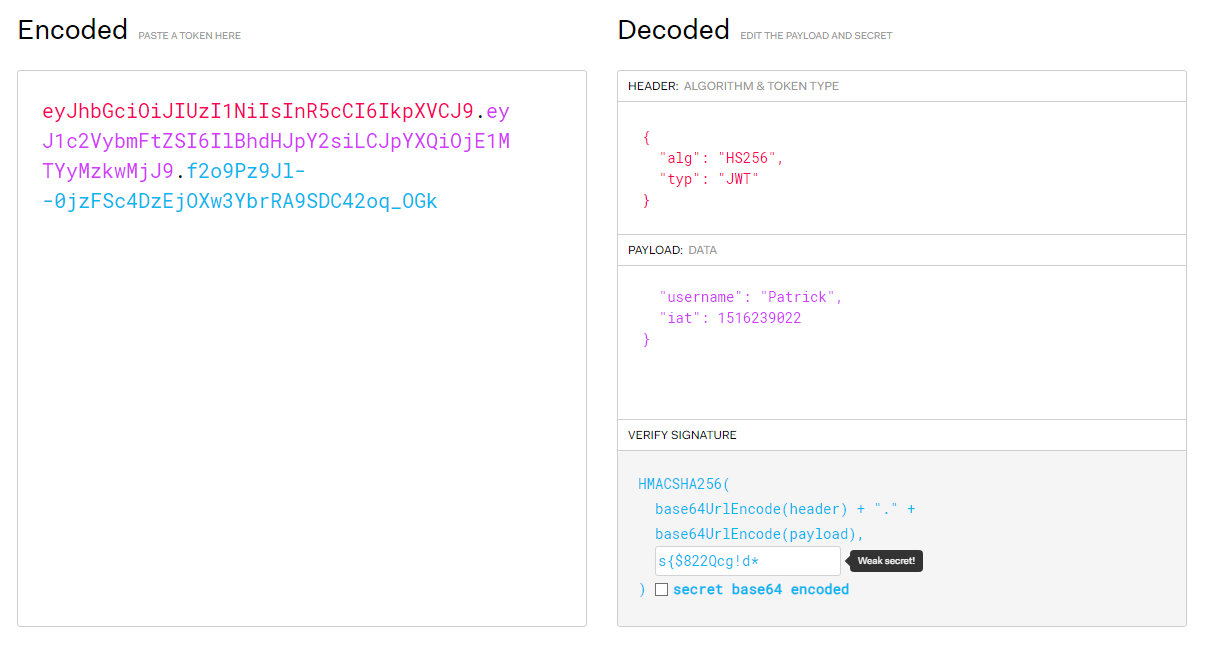
\includegraphics[width=\textwidth]{JWT_Decode.png} % Replace with your image file
    \caption{An example of a decoded JWT}
    \label{fig:example}
\end{figure}
When creating the Wordle app, it became apparent that there would need to be some sort of verification between the front and back end that the user that was set into the user UseState was the actual user logged in. After some research, Java Web Tokens were implemented into the website. With this, the payload would be the username encoded using a public/private key pair and stored in the user's local storage. Whenever a backend function call is made, the JWT is sent to the headers and decoded in the back end to verify the correct user. The username is then pulled from the JWT and used in many function calls to draw the correct user from the database.

\subsection{Keyboard}
During the early stages of the web app, when only the game's logic was in place, it became clear how vital the keyboard was to the “game feel” of Wordle. The keyboard not only gives users the ability to type in their guesses but also helps them keep track of the game's current state. When users have an idea for their next guess, they refer to the keyboard to see which one they have already tried. Without the keyboard, a user has to refer back to their guesses, which is frustrating and challenging to keep track of. 
The keyboard is relatively simple to implement. It passes information into a critical component, such as the letter it should submit, into the input box. It also passes the state of the key to the element, so the colour is updated for each guess. 

\subsection{WordleN}
\begin{lstlisting}[style=python, caption={The setWordLength handler function}]
const handleSetWordLength = (length) => {
        console.log("Setting Word Length " + length)
        setWordLength(parseInt(length));
        setDisabled2(true);
        setShowKeyboard(true);
        createGame(length)
        console.log('Word Length Set')
      };
    const backspace = () => {
        setGuess(guess.slice(0, -1))
    }
\end{lstlisting}
WordleN is a part of the efforts to increase the functionality of the Wordle application. In this component, the user can set a different word length of six, seven, or eight-letter words to increase the level of challenge. The logic is, of course, very similar to the main Wordle component. However, during personal testing in the production phase, it became clear that six guesses to find the solution of an eight-letter word would require more work for users. The solution is that you get an extra guess with each additional letter you must guess, meaning that eight-letter words give you nine guesses. Fortunately, the already implemented code for Wordle accounted for this and will still display guesses until the loss useState is updated. 

\subsection{Navbar}
A navbar is implemented on each application webpage for ease of use. This also uses the router function. The main challenges faced when implementing the navbar were only showing links to the pages that the user had access to and having an active breadcrumb to show which page was currently active. 
The solution to the first issue was very similar to what is done in the app structure. The Navbar also uses ternary operators based on whether the user is logged in. Even if the navbar still displayed the links to other application pages, users would be redirected if they weren’t logged in. However, for clarity’s sake, it is critical to display to the user the parts they can use depending on whether they are logged in. 
The answer to creating a breadcrumb is using the useLocation library provided by React. Each time the component mounts, a LocationProvider constant is created and passed to the navbar. A CSS class then adjusts the button's colour depending on the location.

\subsection{Wordle Frontend}
\begin{lstlisting}[style=python, caption={The loop that updates the results when they are received so they can be placed in the JSX}]
setResult(data.map(previousGuess => {
    let tempData = {
    }
    for (let i = 0; i < 5; i++) {
            let currentLetter = previousGuess.guess.charAt(i).toUpperCase()
            console.log(currentLetter)
            tempData["l"+ i] = {"letter": currentLetter,"result": previousGuess.result[i]}
            console.log(tempData)
            setKeyDictionary(keyDictionary.map(entry => {
                if (entry.key.toUpperCase() === currentLetter){
                    entry.state = previousGuess.result[i]
                }
                console.log(entry)
                return entry
            }))
    }
\end{lstlisting}
When the Wordle component mounts, a useEffect requests the backend to create a game for the user. This call will show no visual change to the component if the user is not in a game. Instead, it will just provide the new game ID within the database. If the user has a game currently active, the frontend will receive the user's previous guesses for that game with the correct labelling if the letter is either “correct”, “present”, or “absent”. This will then be displayed in the JSX as a table with the current guesses and the correct colour to indicate the state of the game. The colouring is done using CSS classes indicated to the front end, depending on what the dictionary returns each letter as.
When a user makes a guess inside the text box, the backend is requested to indicate the updated state of the game. This, in turn, updates the JSX displayed on the page by adding another row to the table with their guess printed out and colouring for each letter, indicating what state the letter is in.
When a user has reached a finished state in the game, whether they have won or not, a modal box is displayed asking if they wish to play again. If they do, the page doesn’t reload; instead, it resets all the useStates within the react component and clears the table of guesses. This modal box also allows users to share the word that they have just tried to guess and send it to another user. 

\subsection{Wordle Backend}
\begin{lstlisting}[style=python, caption={The parseResult function}]
def parseResult(guess, answer):
    confirmed_correct = [''] * len(answer)
    result = []
    letterCount = {}

    for i in range(len(guess)):
        if guess[i] == answer[i]:
            confirmed_correct[i] = guess[i]

    for letter in answer:
        letterCount[letter] = letterCount.get(letter, 0) + 1

    for i, letter in enumerate(confirmed_correct):
        if letter:
            letterCount[letter] -= 1

    for i in range(len(guess)):
        if guess[i] == answer[i]:
            result.append('correct')
        elif guess[i] in answer and letterCount[guess[i]] > 0:
            result.append('present')
            letterCount[guess[i]] -= 1 
        else:
            result.append('absent')

    return result
\end{lstlisting}
The backend will only create a game for the user if they still need to get it in the database with no outcome. In this case, the function creates an entry into the game table of the database with a random answer from the list of words of the correct length and the time the game started. The function returns the gameID to the front end to handle the guess function when the user submits their first guess. Because the leaderboard is tracking a user's average score, it is not appropriate for them to be able to refresh and immediately have a new game. If that were the case, then when the user got to five guesses, they could decide that they don’t believe they can achieve the correct answer, so they could refresh and try again with a new word. The solution to this is to check if they already have a game running without a result in the outcome column of the database. If the user does have a game when the createGame function is called, it is caught, and the backend will return a list of their current guesses, which, in turn, will map their guesses to a table and display it in the front. However, you cannot only send the guesses to the backend as then the words would not have the correct colouring to show whether the letter is in the correct position if it is in the word but not in the correct location, or if the letter is not in the word at all. This is why the parse result function is called in the dictionary and is returned as a JSON object.

How each letter is assigned one of the values, “correct”, “absent”, or “present”, is via the parseResult function. During the initial development of the Wordle component, the parseResult function was relatively simple. The function iterated through each letter of the guessed word, comparing it to the corresponding letter in the correct answer. If the letter in the guess matched the letter at the same position in the answer, it would add "correct" to the result dictionary for that letter. If the letter from the guess was present in the answer but in a different position, it would add "present" to the result dictionary. Otherwise, if the letter were not in the answer, it would be appended as "absent" in the result dictionary. This solution was somewhat functional; however, when put into users' hands, many complained about how letters were marked “present”.
In the original Wordle, if a letter has already been put into the correct position, there was no more of that letter. Suppose the user puts the letter into another position. In that case, it will mark it as “absent,” which created a challenge in creating parity with the original Wordle, which users criticised for making the game unnecessarily difficult. The solution to this was creating a dictionary that stored the number of times each letter was used and, when the letter was found, decreased the count of that letter by one. By doing this, if the letter count of that letter is more significant than zero, you can mark it as present. Otherwise, you mark it as absent.
When a user guesses the text box, a backend function is called, which returns a JSON object that returns each letter with a mark that denotes what colour to use for marking which letters in the word are in the correct position, present in the word but not in the proper position, or absent.
The win/loss state is also created using the backend. Each guess increments the guess count variable, which counts how many entries have been made into the Wordle Guess table with the current game's game ID. If that number reaches one more than the length of the word, giving you six guesses for a five-letter wordle, the game is counted as a loss within the database, and the time you lost is also logged. The function then calls the achievement checker function and rewards you accordingly. The guess function also checks whether the guess received from the front end is the same as the answer. In this case, the database will log the game as a win and the time you finished the game.

\subsection{Achievements Frontend}
The front end of achievements is a table formed from the two JSON objects returned from the backend. When the component is mounted, two separate backend calls are made. These backend calls are separate to pull a list of all the achievements, and then a call is made to send which achievements a user has received. It is then indexed in alphabetical order. The colour, which indicates whether you have received the achievement, is changed depending on which call the achievement came from. 

\subsection{Achievements Backend}
\begin{lstlisting}[style=python, caption={The achievementGetter function.}]
@app.route('/api/achievement_getter', methods=['GET'])
def achievement_getter():
    authoHeader = request.headers.get('authorization')
    print(authoHeader)
    token = authoHeader.split(" ")[1]
    try:
        decodedJwt = jwt.decode(token, "s{$822Qcg!d*", algorithms=["HS256"])
        user = User.query.filter_by(username=decodedJwt['username']).first()
        achievements = UserAchievement.query.filter_by(user_id=user.user_id).all()
        return jsonify ([achievement.achievement.name for achievement in achievements])
    except:
        print(traceback.format_exc())
        return jsonify({"error": "Invalid token"}), 400
\end{lstlisting}
The functionality for achievements in the back end is split into three different functions: one for checking achievements that are called when an outcome is decided for each game, another for sending the user's current achievements to the front end, and one for sending a complete list of achievements to the front end. The latter two are calls made in SQLAlchemy. The first is searching for all the achievements listed in the UserAchievement table matched on the userID fed to the function. The second searches for a complete list of achievement names in the achievements table. 
The achievement checker is more complex as the achievements must be checked differently. We first have to check the user's total wins and losses, both done through calls to SQLAlchemy. Then, the function checks the score of the current game and the time that has been fed to the function. It also tracks averages and creates the game time by removing the end time from the start time. This information is then used to loop through the list of achievements and check whether the user has achieved the achievements with basic logic operators. If the user has completed the achievement and has yet to test it in the User Achievement table, it is appended to a list that is returned when the function is finished. The function then bulk saves the objects added to userAchievements and returns the list. 

\subsection{Leaderboard Frontend}
The leaderboards are returned from the backend and almost fully formed inside the JSON object. These backend calls are stored in a useEffect so that the server will be called as soon as the component mounts. The data is stored in separate useStates when returned from the backend and mapped into JSX elements to be displayed to the user. 

\subsection{Leaderboard Backend}
\begin{lstlisting}[style=python, caption={The Leaderboard SQL call}]
WITH scored_games AS (
    SELECT g.game_id, g.user_id, COUNT(1) AS score, g.start_time, g.end_time
    FROM games g 
    INNER JOIN wordle_guess w ON w.game_id = g.game_id
    WHERE g.outcome IS NOT NULL
      AND LENGTH(g.answer) = 5
    GROUP BY g.game_id, g.user_id, g.start_time, g.end_time
)
SELECT u.firstname,
       ROUND(AVG(g.score), 2) AS score,
       ROUND(AVG(EXTRACT(EPOCH FROM g.end_time) - EXTRACT(EPOCH FROM g.start_time)), 2) AS avg_time,
       RANK() OVER (
           ORDER BY ROUND(AVG(g.score), 2) ASC, 
                    ROUND(AVG(EXTRACT(EPOCH FROM g.end_time) - EXTRACT(EPOCH FROM g.start_time)), 2) ASC
       ) AS rank
FROM users u
INNER JOIN scored_games g ON u.user_id = g.user_id
GROUP BY u.firstname
ORDER BY score, avg_time;
\end{lstlisting}
The leaderboards are created through an SQL query that joins Wordle Guess and the games table. The call then tracks the average score from all users' games and figures out the average length of time a Wordle game takes them. This table is then joined to the user's table from the userID and grouped by the user's first name. It is then ordered by score, and if there is a tie-in score, it is decided by the average time it takes them to complete a Wordle. All the back end does for this is execute the query and return it to the front end in the JSON object. It has to call this query multiple times, with the only adjustment being the length of the answer. This is done so there can be separate leaderboards for each length of Wordle word that can be played. 

\subsection{Share Frontend}
\begin{lstlisting}[style=python, caption={The Share call used on click}]
const share = async () => {
    try {
        const response = await fetch('/api/createSharedGame', {
            method: 'POST',
            headers: {'Content-Type': 'application/json'},
            body: JSON.stringify({ answer: answer})
        })
        if (response.ok) {
            const data = await response.json();
            navigator.clipboard.writeText(`${window.location.origin}/shared/${data.uuid}`)
            enqueueSnackbar('Link copied to clipboard')
        }
    }
    catch (error) {
        console.error(error)
    }
}
\end{lstlisting}
All that is done to accommodate share functionality is creating a route in a router fragment within the app structure. This will redirect to Wordle or WordleN, depending on which page you got the share link from. The modal box at the end of each game has a share button. When this is clicked, a request is sent to the backend, and with this, the frontend sends the answer. A uuid is then returned to the front end, and the body of the link is created when a user clicks on it.

\subsection{Share Backend}
The backend generates a uuid and creates a game in the SharedGame table in the database. All this table contains is a UUID and an answer. When this link is used, the uuid will be pulled from the link and checked against the SharedGame table. All that is done after this is the row with that uuid is found, and the answer is then sent to the createGame function. When a game is returned to the front end, it will function the same, but the answer will now be the word from the game that the user sent it from.
